\chapter{Studi Literatur}

Bab ini menjelaskan secara umum konsep \textit{language model}, perkembangan representasi teks lintas bahasa mulai dari teknik-teknik terdahulu hingga yang terbaru, detail mengenai \textit{multilingual language model} MutlilingualBERT \& XLM-R yang digunakan, metrik evaluasi, dan penelitian terkait. 

\section{Language Model}
    Bab ini dimulai dengan penjelasan singkat konsep dan perkembangan dalam language model. Kemudian diikuti dengan detail arsitektur, teknik, dan pelatihan di pengembangan language model terbaru.

    \subsection{Sejarah Singkat Language Model}
    Representasi dari sebuah bahasa adalah komponen yang sangat penting dalam berbagai penyelesaian masalah bahasa alami secara komputasi. Pendekatan paling sederhana, \textit{one-hot-vector},  merepresentasikan sebuah kalimat berdasarkan ada atau tidaknya sebuah kata. Representasi seperti ini memiliki kekurangan tidak diperhatikannya letak kata dan membesarnya representasi kata seiring membesarnya kosa kata. Kekurangan ini diselesaikan oleh kombinasi \textit{word embedding} dan model sekuensial. 
    
    Salah satu contoh \textit{word embedding} adalah Word2vec \parencite{MikolovWord2vec}. Word2vec yang mempelajari representasi kata sebagai vektor bernilai riil. Tetapi kelemahan pemrosesan teks dengan \textit{word embedding} adalah masih dangkalnya representasi. Representasi \textit{word embedding} tidak dapat menangkap interaksi antar kata di kalimat yang kompleks. Oleh karena itu berkembang teknik \textit{language modelling} terbaru yang memanfaatkan model sekuensial untuk memproses seluruh kalimat dan objektif pelatihhan yang berbeda. 

    Menurut definisi \parencite{Goldberg_2017}, \textit{language modelling} adalah penetapan probabilitas bagi sebuah kalimat di suatu bahasa. Selain menetapkan probabilitas untuk setiap urutan kata, \textit{language model} juga menetapkan probabilitas untuk kemungkinan sebuah kata tertentu (atau sebuah urutan kata) mengikuti urutan kata-kata lainnya. Penelitian terbaru dalam bidang ini memanfaatkan teknik-teknik \textit{neural network} untuk mempelajari probabilitas tersebut.

    Salah satu \textit{language model} terbaru adalah ELMo oleh \parencite{Peters_Neumann_Iyyer_Gardner_Clark_Lee_Zettlemoyer_2018}. Dalam penelitiannya, ia menggunakan model sekuens \text{Long Short-Term Memory} (LSTM) \parencite{Hochreiter_Schmidhuber_1997} \text{bidirectional} sebagai salah satu komponen utama pelatihan. Model dilatih untuk memprediksi token selanjutnya dari sebuah sekuens token. Keterbatasan utama dari model ini adalah fakta bahwasanya model hanya bisa belajar dari satu arah saja pada satu saat. Hal ini diatasi oleh \parencite{Devlin_Chang_Lee_Toutanova_2019} dengan solusinya menggabungkan sekaligus arsitektur transformer dan objektif pelatihan \textit{Masked Language Modeling}. Subbab selanjutnya akan membahas dengan lebih detil hal-hal yang menjadi komponen utama dari pelatihan dan pemanfaatan \text{language model} terbaru oleh \parencite{Devlin_Chang_Lee_Toutanova_2019}.

    \subsection{Arsitektur Transformer}
    Berdasarkan \parencite{AttentionVaswani2017}, arsitektur \textit{Transformer} terdiri dari \textit{self-attention} dan \textit{point-wise} yang ditumpuk, dan \textit{fully connected layer} untuk enkoder dan dekoder. Ilustrasi secara keseluruhan arsitektur \textit{Transformer} dapat dilihat pada Gambar \ref{fig:ilustrasi_transformer}.

    \begin{figure}[ht]
        \centering
        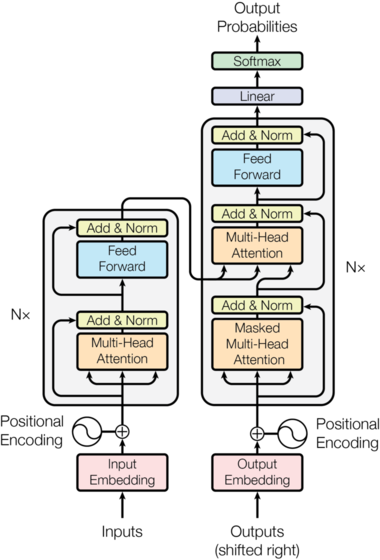
\includegraphics[width=0.4\textwidth]{resources/overview-transformer.png}
        \caption{Ilustrasi \textit{transformer} secara keseluruhan \parencite{AttentionVaswani2017}.}
        \label{fig:ilustrasi_transformer}
    \end{figure}

    Fungsi \textit{attention} dapat digambarkan sebagai memetakan kueri dan pasangan \textit{key-value} untuk suatu output, di mana kueri (Q), kunci (K), nilai (V), dan \textit{output} semuanya vektor. \textit{Output} dihitung sebagai \textit{weighted sum} dari nilai-nilai, di mana bobot yang ditetapkan untuk setiap nilai dihitung oleh fungsi kompatibilitas kueri dari kunci yang sesuai.

    Pada penelitian \parencite{AttentionVaswani2017}, tipe \textit{attention} ini disebut "\textit{Scaled Dot-Product Attention}". Input terdiri dari kueri dan kunci dimensi \(d_{k}\), dan nilai dimensi \(d_{v}\). \textit{Dot product} dari kueri dihitung dengan semua kunci, membaginya dengan \(\sqrt{d_{k}}\), dan menerapkan fungsi softmax untuk mendapatkan bobot pada nilai. Ilustrasi \textit{attention} dapat dilihat pada Gambar \ref{fig:ilustrasi_attention}.

    \begin{figure}[ht]
        \centering
        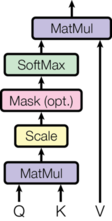
\includegraphics[width=0.2\textwidth]{resources/overview-attention.png}
        \caption{Ilustrasi \textit{attention} secara keseluruhan \parencite{AttentionVaswani2017}.}
        \label{fig:ilustrasi_attention}
    \end{figure}

    Pada prakteknya, hasil keluaran fungsi \textit{attention} pada sebuah set kueri dihitung secara besamaan, dikemas bersama menjadi matriks Q. Kunci dan nilai juga dikemas bersama menjadi matriks K dna V. Kemudian hasil keluaran dapat dihitung dengan:

    \begin{equation}
        Attention(Q,K,V) = softmax(\frac{QK^{T}}{\sqrt{d_k}})V
    \end{equation}

    Pada model MultilingualBERT dan XLM-R yang digunakan di tugas akhir ini, arsitektur Transformer menjadi kunci utama desain model. Model MultilingualBERT terdiri dari 12 blok layer Transformer, 768 \textit{hidden size}, 12 \textit{self-attention heads}, 110 ribu kosa kata, dan total 172 juta parameter. Lalu, model XLM-R Base terdiri dari terdiri dari 12 blok layer Transformer, 768 \textit{hidden size}, 12 \textit{self-attention heads}, 250 ribu kosa kata, dan total 270 juta parameter. Terakhir, model XLM-R Large terdiri dari terdiri dari 24 blok layer Transformer, 1024 \textit{hidden size}, 16 \textit{self-attention heads}, 250 ribu kosa kata, dan total 550 juta parameter.

    \subsection{Masked Language Modeling (MLM)}
    Dideskripsikan pertama kali pada penelitian \parencite{Devlin_Chang_Lee_Toutanova_2019}, \textit{Masked Language Modeling} terinspirasi dari \textit{Cloze task} \parencite{Taylor_1953}. Teknik MLM secara acak menyembunyikan beberapa kata dari input, dan model memiliki objektif untuk menebak kata asli dari kata yang disembunyikan tadi berdasarkan konteks yang ada di sekelilingnya. Tidak seperti pelatihan \textit{language model} lainnya yang berjalan dari kiri-ke-kanan, pelatihan dengan objektif MLM memungkinkan representasi dari kiri dan kanan mengambil peran. Hal ini memungkinkan pelatihan \textit{Transformer} secara dua arah. Ilustrasi dari \textit{masked language modeling} secara keseluruhan dapat dilihat pada Gambar \ref{fig:ilustrasi_mlm}.

    \begin{figure}[ht]
        \centering
        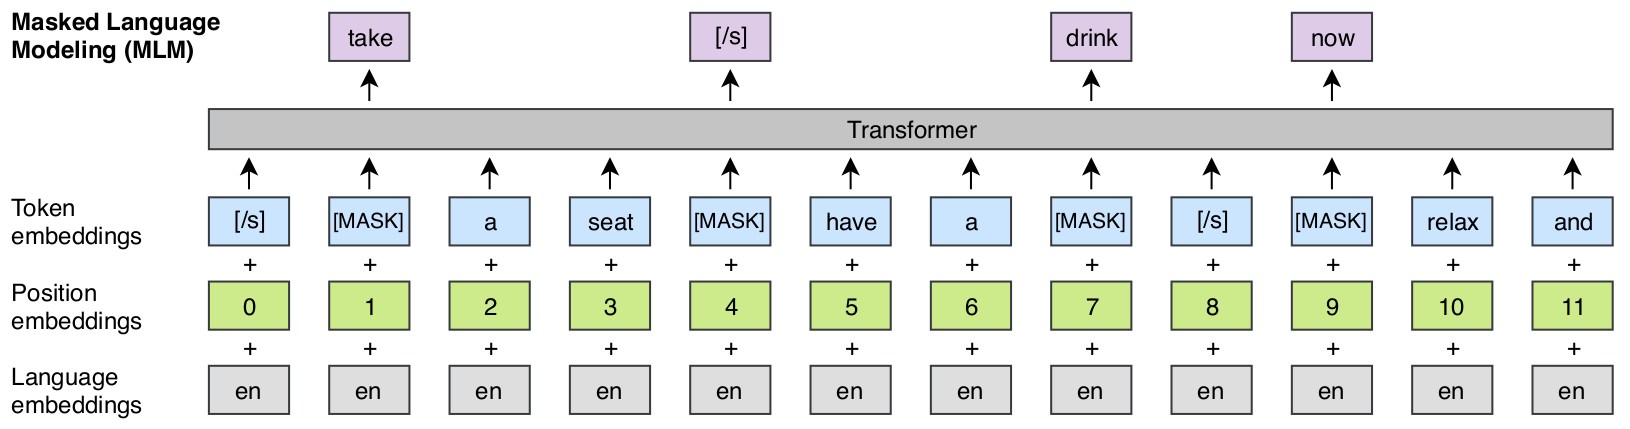
\includegraphics[width=1\textwidth]{resources/ilustrasi-mlm.png}
        \caption{Ilustrasi \textit{masked language modeling} \parencite{LampleConneau2019}.}
        \label{fig:ilustrasi_mlm}
    \end{figure}

    Sama dengan BERT, persentase dari kata yang dipilih untuk disembunyikan pada XLM adalah 15 persen. Setelah sebuah posisi dipilih secara acak, sebuah kata kemudian memiliki 80 persen kemungkinan untuk disembunyikan, 10 persen kemungkinan untuk diganti menjadi sebuah kata acak, dan 10 persen kemungkinan tidak diganti sama sekali.

    \subsection{Teknik Pretraining}
    Model BERT dan XLM merupakan perkembangan dari penelitian oleh \parencite{radford2018improving} dan \parencite{HowardRuder2018} yang meneliti \textit{language modeling} untuk melakukan \textit{pretraining Transformer encoder}. Penelitian-penelitian tersebut sukses membuktikan mangkusnya teknik ini dengan meraih kenaikan performa yang tinggi pada dataset tolak ukur GLUE \parencite{GLUE2019}.

    Teknik \textit{language model pretraining} sukses dikarenakan kemampuannya untuk memanfaatkan data-data teks yang ada dari berbagai sumber tanpa perlu melakukan pelabelan \textit{(unsupervised)}. Pada salah satu model XLM, \textit{pretraining} dilakukan pada data Wikipedia dari 100 bahasa. Melalui pembelajaran dari Wikipedia 100 bahasa ini XLM berhasil mempelajari representasi teks berbagai bahasa.

	\subsection{Teknik Fine-tuning}
	Untuk melakukan \textit{fine-tuning} model klasifikasi teks biner, sebuah \textit{dense layer} ditambahkan di atas keluaran dari \textit{language model} yang sudah di-\textit{pretrained}. Hal ini sama dengan teknik yang \parencite{LampleConneau2019} lakukan pada masalah klasifikasi antar bahasa dengan dataset XNLI \parencite{Conneau_Rinott_Lample_Williams_Bowman_Schwenk_Stoyanov_2018}. Penelitian, \parencite{Devlin_Chang_Lee_Toutanova_2019} mendefinisikan dua teknik \textit{fine-tuning} yang biasa dilakukan adalah melatih keseluruhan model atau hanya menggunakan \textit{language model} untuk mengekstraksi fitur dan kemudian melatih layer terakhir saja. Berikut penjelasan dan ilustrasi mengenai dua teknik tersebut
	\begin{enumerate}
		\item \textbf{Hanya Layer Terakhir}\\	
		Melatih	model secara keseluruhan memerlukan waktu dan sumber daya yang besar. Waktu dapat dipersingkat dengan membekukan dan tidak melatih lebih lanjut komponen \textit{multilingual language model} yang sudah mempelajari representasi teks antar bahasa. Komponen yang dilatih hanyalah \textit{dense layer} yang baru ditambahkan di atas model untuk melakukan klasifikasi. Ilustrasi dari proses ini dapat dilihat pada Gambar \ref{fig:ilustrasi_head_fine_tune}.

        Teknik \textit{fine-tuning} seperti ini memang menghasilkan performa yang lebih rendah dibanding melakukan \textit{fine-tuning} penuh seluruh arsitektur. Hal ini dikarenakan penggunaan representasi teks lintas bahasa yang murni dari hasil \textit{pretraining} sebagai fitur dan tidak dilakunannya penyempurnaan representasi ke permasalahan yang sedang diselesaikan. Tetapi walaupun begitu, efek dari penggunaan \textit{multilingual language model} dalam memanfaatkan bahasa yang lebih banyak sumber dayanya ke permasalahan bahasa Indonesia tetap dapat diobservasi.
        
        \begin{figure}[h]
            \centering
            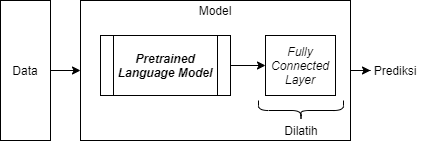
\includegraphics[width=0.75\textwidth]{resources/Head-fine-tune.png}
            \caption{ Ilustrasi \textit{fine-tuning} layer terakhir}
            \label{fig:ilustrasi_head_fine_tune}
        \end{figure}

		\item \textbf{Penuh}\\
        Pada teknik \textit{fine-tuning} full, seluruh arsitektur dilatih dengan fungsi \textit{loss} dari hasil klasifikasi. Dengan teknik ini, potensi secara keseluruhan dari \textit{pretrained multilingual language model} dapat diobservasi. Ilustrasi dari proses ini dapat dilihat pada Gambar \ref{fig:ilustrasi_full_fine_tune}.
        
        \begin{figure}[h]
            \centering
            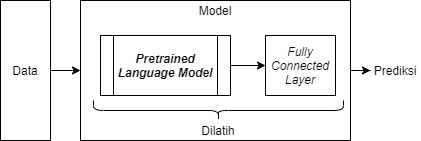
\includegraphics[width=0.75\textwidth]{resources/Full-fine-tune.png}
            \caption{ Ilustrasi \textit{fine-tuning} penuh}
            \label{fig:ilustrasi_full_fine_tune}
        \end{figure}
		
	\end{enumerate}

\section{Representasi Teks Lintas Bahasa}
    Representasi teks lintas bahasa diperlukan untuk dapat memanfaatkan bahasa Inggris dalam melatih model untuk klasifikasi teks bahasa Indonesia. Representasi teks lintas bahasa berarti merepresentasi bahasa pada ruang yang sama seperti dapat dilihat pada ilustrasi di gambar \ref{fig:ilustrasi_embedding}.

    \begin{figure}[ht]
        \centering
        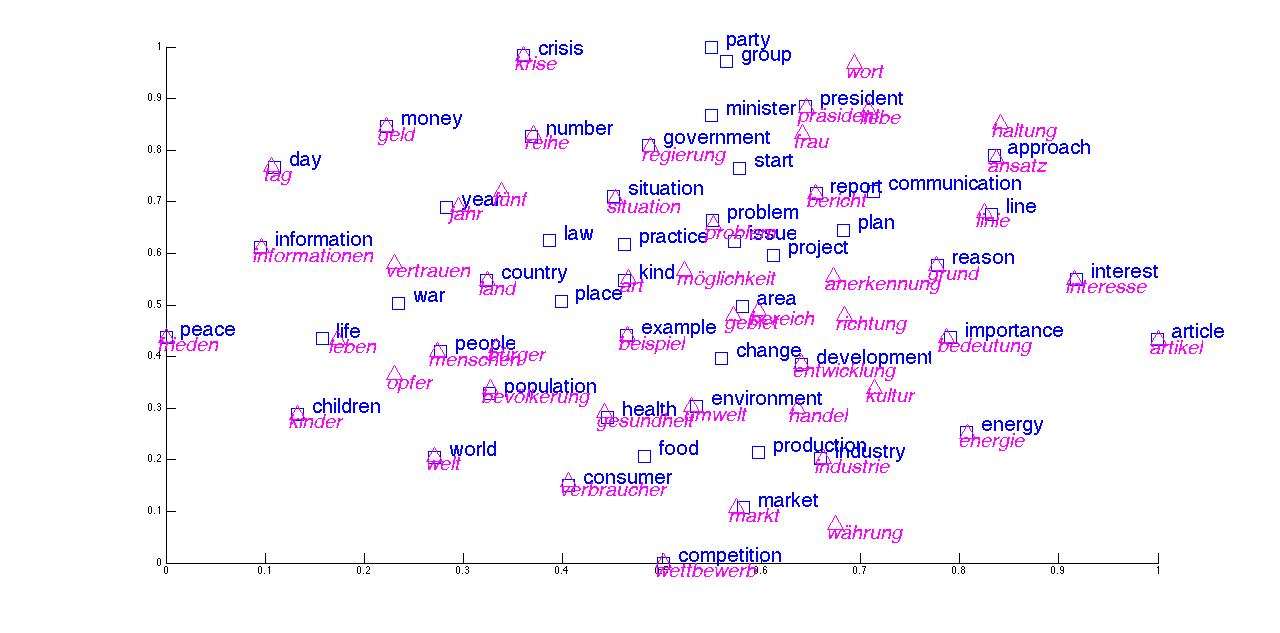
\includegraphics[width=1\textwidth]{resources/luong_et_al_2015.jpg}
        \caption{Ilustrasi ruang \textit{embedding} antara dua bahasa \parencite{Luong_Pham_Manning_2015}} 
        \label{fig:ilustrasi_embedding}
    \end{figure}

    Sebelumnya, diperlukan ahli untuk membangun kamus kata-kata dan kalimat secara manual untuk dapat membandingkan kata dari dua bahasa. Seiring dengan perkembangan teknologi, berbagai teknik berkembang untuk dapat melakukan hal ini secara otomatis. Berdasarkan \parencite{Wang_Xie_Xu_Yang_Neubig_Carbonell_2019}, secara garis besar terdapat 2 pendekatan berbeda dalam membangun ruang \textit{embedding} antar bahasa: \textit{monolingual mapping} dan \textit{joint optimization}. Subbab selanjutnya akan membahas dua hal tersebut.

    \subsection{Monolingual Mapping}

    Pada \textit{monolingual mapping},  model dilatih secara independen pada bahasa masing-masing. Kemudian mapping antara bahasa dipelajari untuk mendapatkan representasi antar bahasa. Salah satu contohnya adalah penelitian \parencite{MikolovEstimation}. Pada penelitiannya pertama-tama dipelajari representasi bahasa menggunakan model Skip-gram atau Continuous Bag-of-Words (CBOW) yang didistribusikan. Model-model ini mempelajari representasi kata menggunakan arsitektur \textit{neural network} sederhana yang bertujuan untuk memprediksi tetangga kata. Karena kesederhanaannya, model Skip-gram dan CBOW dapat dilatih pada sejumlah besar data teks. Pada implementasi paralelnya model ini dapat belajar dari miliaran kata dalam hitungan jam.

    Baru-baru ini ditunjukkan bahwa representasi kata yang didistribusikan secara mengejutkan menangkap banyak keteraturan linguistik, dan ada banyak jenis kesamaan di antara kata-kata yang dapat dinyatakan sebagai terjemahan linear \parencite{MikolovLinguistic2013}. Misalnya, operasi vektor "raja" - "pria" + "wanita" menghasilkan vektor yang dekat dengan "ratu".

    Dua model khusus untuk mempelajari representasi kata yang dapat dilatih secara efisien pada banyak data teks adalah model Skip-gram dan CBOW yang diperkenalkan di \parencite{MikolovEstimation}. Dalam model CBOW, tujuan pelatihannya adalah untuk menggabungkan representasi kata di sekitarnya untuk memprediksi kata di tengah. Sedangkan dalam model Skip-gram, tujuan pelatihan adalah untuk mempelajari representasi kata vektor yang pandai memprediksi konteksnya dalam kalimat yang sama \parencite{MikolovEstimation}. Model arsitektur dari dua metode ini ditunjukkan pada Gambar \ref{fig:ilustrasi_cbow_skip_gram}.

    \begin{figure}[ht]
        \centering
        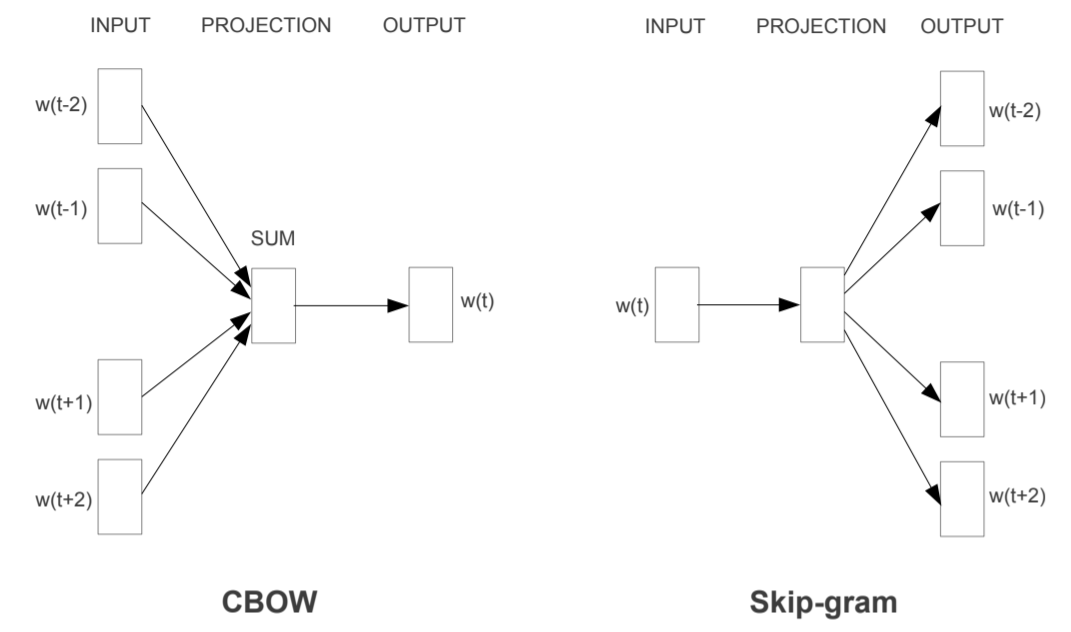
\includegraphics[width=1\textwidth]{resources/cbow-skip-gram-illustration.png}
        \caption{Ilustrasi model CBOW dan Skip-gram. \parencite{MikolovExploiting}.}
        \label{fig:ilustrasi_cbow_skip_gram}
    \end{figure}
    
    Lebih formal, diberi urutan kata pelatihan \(w1, w2, w3,. . . , wT,\) tujuan dari model Skip-gram adalah untuk memaksimalkan probabilitas log rata-rata

    \begin{equation}
        \frac{1}{T}\sum_{t=1}^{T}\begin{bmatrix}
        \sum_{j=-k}^{K}{\log p(w_{t+j}|w_{t})}
        \end{bmatrix}
        \label{eq:1}
    \end{equation}

    di mana \(k\) adalah ukuran jendela pelatihan. Iterasi penjumlahan di bagian dalam berjalan dari \({-k}\) ke \(k\) untuk menghitung probabilitas log benarnya memprediksi kata \(w_{t+j}\) jika kata di tengah \(w_{t}\). Iterasi penjumlahan di luar mencakup semua kata dalam korpus pelatihan. 

    Ketika dilatih tentang dataset besar, model Skip-gram atau CBOW ini menangkap banyak informasi semantik. Seperti yang disebutkan sebelumnya, kata-kata yang berkaitan erat memiliki representasi vektor yang serupa, misalnya, sekolah dan universitas, danau, dan sungai. Ini karena sekolah dan universitas muncul dalam konteks yang sama, sehingga selama pelatihan representasi vektor dari kata-kata ini didorong untuk menjadi dekat satu sama lain. Lebih menarik lagi, vektor menangkap hubungan antara konsep melalui operasi linier. Misalnya, \(vektor(Prancis) - vektor(Paris)\) mirip dengan \(vektor(Italia) - vektor(Roma)\).

    Pada gambar \ref{fig:ilustrasi_embedding_inggris_spanyol}, dapat dilihat visualisasi hasil pembelajaran Skip-gram atau CBOW. Gambar \ref{fig:ilustrasi_embedding_inggris_spanyol} memvisualisasikan vektor untuk angka dan hewan dalam bahasa Inggris dan Spanyol, dan dapat dengan mudah dilihat bahwa konsep-konsep ini memiliki susunan geometris yang serupa. Hal ini dikarenakan semua bahasa umum memiliki konsep yang didasarkan pada dunia nyata (seperti kucing adalah binatang yang lebih kecil dari seekor anjing), sering kali ada kesamaan kuat antara ruang vektor. Kesamaan pengaturan geometris dalam ruang vektor adalah alasan utama mengapa metode ini dapat bekerja dengan baik.

    \begin{figure}[ht]
        \centering
        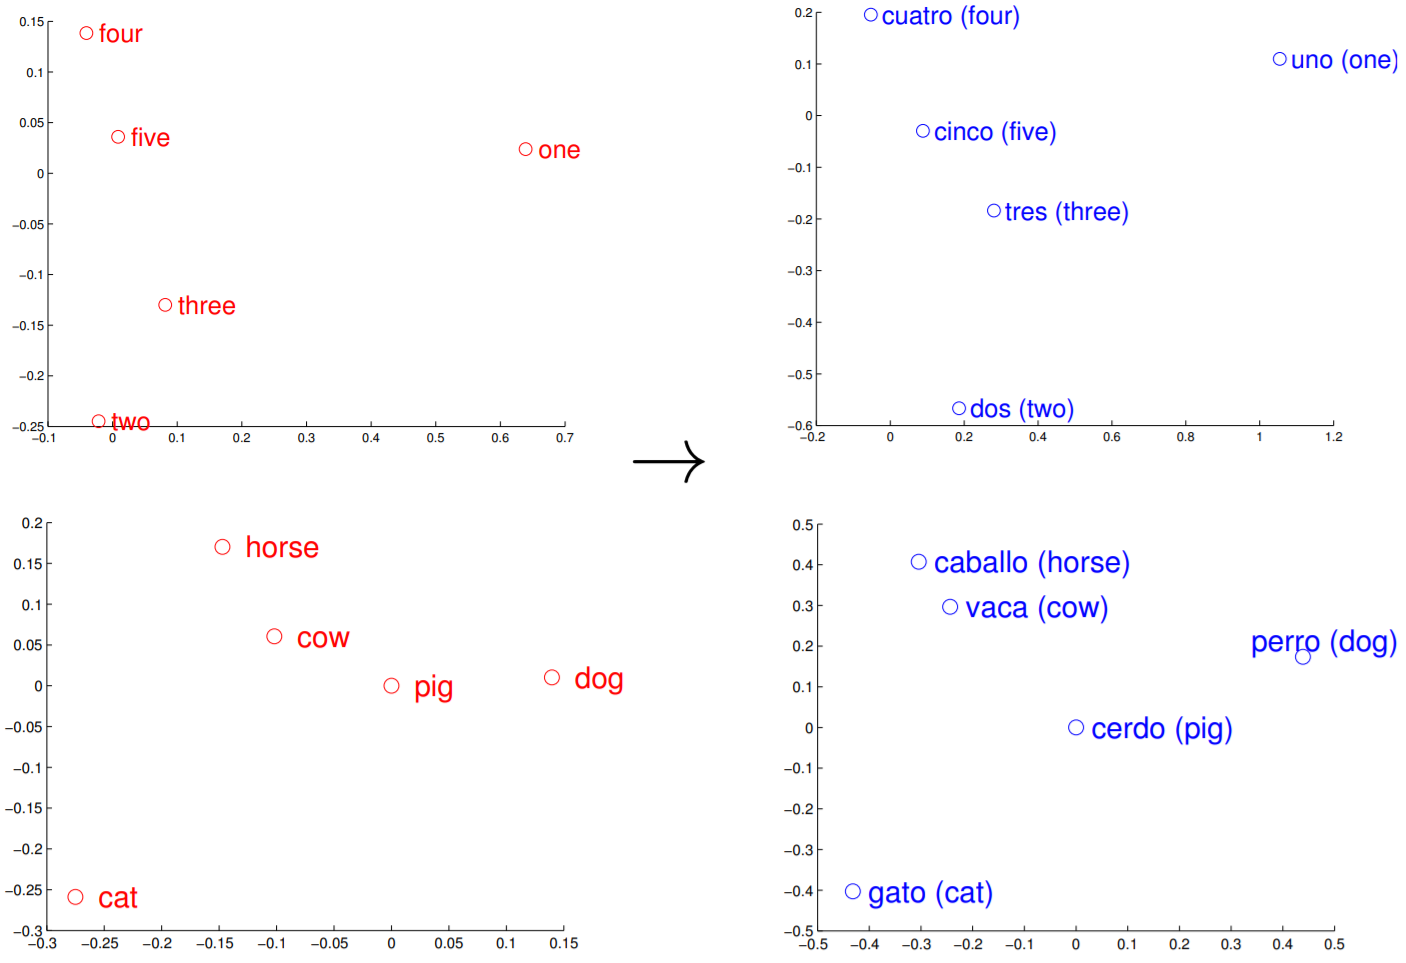
\includegraphics[width=1\textwidth]{resources/ilustration-eng-spn-word.png}
        \caption{Ilustrasi ruang \textit{embedding} antara bahasa Inggris dan Spanyol \parencite{MikolovExploiting}.}
        \label{fig:ilustrasi_embedding_inggris_spanyol}
    \end{figure}

    Dikarenakan miripnya representasi bahasa, jika translasi beberapa objek diketahui, contoh angka satu sampai lima, representasi antar bahasa dapat disesuaikan dengan rotasi, \textit{scaling}, dan translasi untuk mendapatkan translasi angka lainnya. Lebih formalnya, misalkan diberi satu set pasangan kata dan representasi vektor yang terkait \begin{math} \begin{Bmatrix} {x_{i}, z_{i}} \end{Bmatrix}_{i=1}^{n} \end{math}, di mana \(x_{i}\in\mathbb{R}^{d_{1}}\) adalah representasi terdistribusi dari kata i dalam bahasa sumber, dan \(z_{i}\in\mathbb{R}^{d_{2}}\) adalah representasi vektor dari terjemahannya. Kemudian dicari matriks transformasi \( W\) sehingga \(W x_{i}\) mendekati \(z_{i}\). Dalam praktiknya, \(W\) dapat dipelajari dengan masalah optimasi berikut

    \begin{equation}
        \min_{W}\sum_{i=1}^{n}\left \| Wx_i-z_i \right \|^2
        \label{eq:2}
    \end{equation}

    yang dapat diselesaikan dengan \textit{stochastic gradient descent} \parencite{MikolovExploiting}.

    Setiap kata baru yang diberikan dan representasi vektor kontinu \(x\) dapat dipetakan ke ruang bahasa lain dengan menghitung \(z = W x\) pada saat prediksi. Kemudian kata yang representasinya paling dekat dengan \(z\) dalam ruang bahasa target dapat ditemukan menggunakan \textit{cosine similarity} sebagai metrik jarak. Terlepas dari kesederhanaannya, metode transformasi linier ini bekerja dengan baik dalam eksperimen yang \parencite{MikolovExploiting} jalankan, lebih baik daripada teknik \textit{nearest neighbour} dan juga pengklasifikasi \textit{neural network}.

    Meski \textit{monolingual mapping} sukses mendapatkan ruang \textit{embedding} antar bahasa, teknik ini mahal dan susah diaplikasikan ke bahasa yang memiliki sumber daya rendah. Untuk dapat mengaplikasikan teknik ini diperlukan kamus kata-kata atau kalimat paralel antar bahasa, hal yang seringkali tidak tersedia pada bahasa bersumber daya rendah. Oleh karena itu, mengaplikasikan teknik ini sangat sulit pada bahasa Indonesia.
    
    \subsection{Joint Optimization}
    Pada teknik \textit{Joint Optimization}, model dilatih pada korpus dari berbagai bahasa. Model kemudian mengoptimisasi \textit{loss} dari objektif monolingual, \textit{cross-lingual}, atau kombinasi keduanya. Sebuah kemajuan terbaru dari teknik \textit{joint optimization} berhasil mengatasi permasalahan dibutuhkannya kamus paralel yang ada di teknik sebelumnya. Teknik \textit{joint optimization} yang sebelumnya memerlukan korpus paralel atau kamus bilingual (\textit{supervised}) \parencite{Xing_Wang_Liu_Lin}, kini dapat dilakukan tanpa korpus paralel atau kamus bilingual (\textit{unsupervised}) \parencite{Devlin_Chang_Lee_Toutanova_2019} \parencite{LampleConneau2019}. Penelitian \parencite{Devlin_Chang_Lee_Toutanova_2019} dan \parencite{Conneau_XLMR} melatih model pada korpus dari berbagai bahasa tanpa menggunakan objektif \textit{cross-lingual} apapun. Model yang dihasilkan telah menunjukkan kemampuan generalisasi yang baik di seluruh bahasa dan representasi agnostik bahasa di dalam keadaan tersembunyi \parencite{Pires_Schlinger_Garrette_2019}.

    Hingga saat ini, penjelasan mengenai kenapa teknik ini bekerja dengan sangat baik dalam menghasilkan representasi antar bahasa masih menjadi penelitian. Salah satu hipotesis mengenai kenapa representasi antar bahasa tersebut dapat diraih tanpa objektif antar bahasa adalah penggunaan \textit{sub-word}. Berdasarkan penelitian oleh \parencite{Sennrich_Haddow_Birch_2016}, salah satu inspirasi menggunakan \textit{sub-word} adalah fakta bahwa terjemahan beberapa kata bersifat transparan karena terjemahannya dapat diterjemahkan oleh penerjemah yang kompeten, bahkan jika itu adalah kata yang belum pernah ditemui, berdasarkan terjemahan dari \textit{sub-word} yang dikenal seperti morfemnya atau fonemnya. Kategori kata yang terjemahannya berpotensi transparan meliputi:

    \begin{enumerate}
        \item Entitas bernama (\textit{named entities}). Di antara bahasa yang menggunakan alfabet, nama seringkali dapat disalin dari sumber ke teks target. Transkripsi atau transliterasi mungkin diperlukan pada bahasa dengan huruf atau suku kata berbeda. Contoh: \\
        Barack Obama (Bahasa Inggris dan Jerman) \\
        \foreignlanguage{russian}{Барак Обама} (Bahasa Rusia) \\
        \begin{CJK}{UTF8}{min}
        バラク・オバマ (ba-ra-ku o-ba-ma) (Bahasa Jepang)
        \end{CJK}

        \item Kata-kata serumpun dan pinjaman. Kata serumpun dan kata pinjaman dengan asal yang sama dapat berbeda secara reguler antar bahasa, sehingga aturan penerjemahan tingkat karakter sudah cukup \parencite{Tiedemann2012}. Contoh:  \\
        claustrophobia (Bahasa Inggris) \\
        Klaustrophobie (Bahasa Jerman) \\
        \foreignlanguage{russian}{Клаустрофобия} (Klaustrofobiâ) (Bahasa Rusia)

        \item Kata-kata yang rumit secara morfologis. Kata-kata yang mengandung banyak morfem, misalnya yang dibentuk melalui peracikan, afiksasi, atau infleksi, dapat diterjemahkan dengan menerjemahkan morfem secara terpisah. Contoh:  \\
        solar system (Bahasa Inggris) \\
        Sonnensystem (Sonne + System) (Bahasa Jerman) \\
        Naprendszer (Nap + Rendszer) (Bahasa Hongaria)
    \end{enumerate}

    Penelitian \parencite{Sennrich_Haddow_Birch_2016} membuktikan bahwa segmentasi kata-kata langka ke dalam unit \textit{sub-word} yang sesuai sudah cukup untuk memungkinkan \textit{neural translation network} mempelajari terjemahan yang transparan, dan menggeneralisasikan pengetahuan ini untuk menerjemahkan dan menghasilkan kata-kata yang tidak ditemui sebelumnya. Pada penelitiannya, mereka menggunakan teknik \textit{Byte Pair Encoding} untuk mendapatkan tidak hanya \textit{sub-word}-nya tetapi juga kompresi dari kamus-kamus kata yang ada.

    Teknik \textit{Byte Pair Encoding} (BPE) \parencite{GageBPE1994} adalah teknik kompresi data sederhana yang secara iteratif menggantikan pasangan \textit{byte} yang paling sering muncu; secara berurutan dengan \textit{byte} tunggal yang tidak digunakan. Pada penelitiannya, \parencite{Sennrich_Haddow_Birch_2016} mengadaptasi algoritma \textit{Byte Pair Encoding} untuk segmentasi kata. Alih-alih sering menggabungkan pasangan \textit{byte}, mereka menggabungkan karakter atau urutan karakter.

    Pertama-tama, kosakata simbol diinisialisasi dengan kosakata karakter, dan mewakili setiap kata sebagai urutan karakter, ditambah simbol akhir kata khusus ‘·’, yang memungkinkan hasil terjemahan dikembalikan ke bentuk awal setelah terjemahan. Kemudian semua pasangan simbol dihitung secara iteratif dan untuk setiap pasangan yang paling sering diganti dengan simbol baru. Contoh ('A', 'B') menjadi 'AB'. Setiap operasi penggabungan menghasilkan simbol baru yang mewakili \textit{n-gram} dari karakter. Karakter yang sering muncul (atau seluruh kata) pada akhirnya digabungkan menjadi satu simbol. Ukuran kosa kata simbol akhir sama dengan ukuran kosa kata awal, ditambah jumlah operasi penggabungan --- yang merupakan satu-satunya \textit{hyperparameter} dari algoritma.

    Dapat dilihat contoh sederhana algoritma \textit{Byte Pair Encoding} pada Lampiran \ref{appendix:simple_bpe_algorithm} oleh \parencite{Sennrich_Haddow_Birch_2016}. Pada algoritma ini, operasi \textit{Byte Pair Encoding} belajar dari kamus kata {‘low’, ‘lower’, ‘newest’, ‘widest’}. Pada akhir iterasi, diperoleh representasi dari kamus kata dalam bentuk simbol-simbol yang dipelajari. Pada contoh tersebut, kata 'lowest' yang berada diluar kamus kata direpresentasikan menjadi gabungan dari simbol 'low' dan 'est'. Di sini dapat dilihat bagaimana \textit{Byte Pair Encoding} dapat membantu merepresentasikan kata yang berada diluar kamus kata. 

    Namun penelitian \parencite{K_Wang_Mayhew_Roth_2020} berhasil mematahkan hipotesis penggunaan \textit{sub-word} ini dengan melatih model menggunakan data yang sama sekali tidak memiliki \textit{sub-word} tumpang tindih. Hasil dari penelitiannya membuktikan bahwa tumpang tindih leksikal antara bahasa memainkan peran yang dapat diabaikan dalam keberhasilan lintas bahasa. Oleh karena itu, penelitian dalam menjelaskan efektifitas teknik ini masih gencar dilakukan.

\section{Multilingual Language Model}
    Bab ini menjelaskan detail dari dua \textit{multilingual language model} yang digunakan dalam tugas akhir ini: MultilingualBERT dan XLM-RoBERTa.

    \subsection{MultilingualBERT}
        MultilingualBERT adalah salah satu model yang penelitian \parencite{Devlin_Chang_Lee_Toutanova_2019} rilis. Model ini pada dasarnya memiliki arsitektur sama dengan varian BERT-Base yang terdiri dari 12 blok layer Transformer, 768 \textit{hidden size}, 12 \textit{self-attention heads}, dan total 110 juta parameter. Hanya saja model ini tidak dilatih dengan data dari BooksCorpus (800 juta kata) dan Wikipedia bahasa Inggris (2,5 miliar kata). Melainkan, model ini dilatih dengan data Wikipedia dari lebih 104 bahasa.
        
        Meski tidak didesain secara eksplisit untuk memiliki representasi antar bahasa, penelitian \parencite{Pires_Schlinger_Garrette_2019} menunjukkan bahwa MultilingualBERT memiliki kemampuan generalisasi antar bahasa yang sangat baik. Pada penelitiannya, \parencite{Pires_Schlinger_Garrette_2019} mendemonstrasikan kemampuan MultilingualBERT pada berbagai permasalahan dan menyiratkan terdapatnya informasi linguistik yang berguna antar bahasa  pada representasi di dalam MultilingualBERT

    \subsection{XLM-RoBERTa}
        XLM-RoBERTa adalah model yang dirilis dari hasil penelitian \parencite{Conneau_XLMR}. Penelitian ini mengembangkan hasil penelitian \parencite{LampleConneau2019} dengan data lebih banyak, data yang lebih beragam, dan teknik pelatihan yang lebih optimal. Model yang dirilis memiliki dua varian, XLM-R Base dan XLM-R Large. Model XLM-R Base terdiri dari terdiri dari 12 blok layer Transformer, 768 \textit{hidden size}, 12 \textit{self-attention heads}, dan total 270 juta parameter. Terakhir, model XLM-R Large terdiri dari terdiri dari 24 blok layer Transformer, 1024 \textit{hidden size}, 16 \textit{self-attention heads}, dan total 550 juta parameter. 

        Meski MultilingualBERT memiliki kemampuan generalisasi antar bahasa, masih terdapat banyak kekurangan yang menghambat kemampuan generalisasi ini maju.
        Penelitian berjudul "RoBERTa: Pendekatan Pretraining BERT yang Lebih Optimal" oleh \parencite{Liu_Ott_Goyal_Du_Joshi_Chen_Levy_Lewis_Zettlemoyer_Stoyanov_2019} menunjukkan bahwa teknik pelatihan dan beberapa pilihan desain dalam pemodelan BERT tidak optimal. Lalu dalam pembangunannya BERT juga tidak didesain dan dioptimisasi secara khusus untuk dapat generalisasi antar bahasa, hal yang \parencite{Conneau_XLMR} teliti dan perbaiki. Subbab selanjutnya membahas beberapa hal tersebut dengan lebih detail.


        \begin{table}[tb]
            \centering
            \caption{Rangkuman perbandingan objektif pelatihan \parencite{Liu_Ott_Goyal_Du_Joshi_Chen_Levy_Lewis_Zettlemoyer_Stoyanov_2019} }
            \begin{tabular}{|l|l|l|l|l|}
                \hline
                \textbf{Model} & \textbf{SQuAD 1.1/2.0} & \textbf{MNLI-m} & \textbf{SST-2} & \textbf{RACE} \\ \hline
                \multicolumn{5}{|l|}{\textit{Dengan NSP Loss:}}                                            \\ \hline
                SEGMENT-PAIR   & 90.4/78.7              & 84.0            & \textbf{92.9}  & 64.2          \\ \hline
                SENTENCE-PAIR  & 88.7/76.2              & 82.9            & 92.1           & 63.0          \\ \hline
                \multicolumn{5}{|l|}{\textit{Tanpa NSP Loss:}}                                             \\ \hline
                FULL-SENTENCES & 90.4/79.1              & \textbf{84.7}   & 92.5           & 64.8          \\ \hline
                DOC-SENTENCES  & \textbf{90.6/79.7}     & \textbf{84.7}   & 92.7           & \textbf{65.6} \\ \hline
            \end{tabular}
            \label{tab:rangkuman_roberta_1}
        \end{table}

        \subsection{Perubahan dari Desain BERT: Next Sentence Prediction dan Static Masking}
        Penelitian \parencite{Liu_Ott_Goyal_Du_Joshi_Chen_Levy_Lewis_Zettlemoyer_Stoyanov_2019} mengevaluasi kembali desain kunci pada pelatihan BERT. BERT memiliki dua objektif pelatihan, \textit{Masked Language Model (MLM)} dan \textit{Next Sentence Prediction (NSP)}. Sedangkan pada cara \textit{masking} data untuk MLM, data di-\textit{mask} secara static. Berarti selama pelatihan, teks yang di-\textit{mask} hanya itu saja dan tidak berubah. Dua Desain kunci ini adalah beberapa hal yang dievaluasi oleh \parencite{Liu_Ott_Goyal_Du_Joshi_Chen_Levy_Lewis_Zettlemoyer_Stoyanov_2019}.

        Pada objektif pelatihan, \parencite{Liu_Ott_Goyal_Du_Joshi_Chen_Levy_Lewis_Zettlemoyer_Stoyanov_2019} membandingkan dengan cermat penggunaan objektif NSP pada berbagai tipe cara memasukkan data kedalam pelatihan model. Hasil perbandingan menunjukkan bahwa penghilangan objektif NSP berefek bagus atau sama saja pada performa model. Rangkuman hasil perbandingan dapat dilihat pada Tabel \ref{tab:rangkuman_roberta_1}.

        \begin{table}[b]
            \centering
            \caption{Rangkuman perbandingan teknik \textit{masking} \parencite{Liu_Ott_Goyal_Du_Joshi_Chen_Levy_Lewis_Zettlemoyer_Stoyanov_2019} }
            \begin{tabular}{lccc}
                \hline
                \textbf{Masking} & \textbf{SQuAD 1.1/2.0} & \textbf{MNLI-m} & \textbf{SST-2} \\ \hline
                \textit{static}  & 78.3                   & \textbf{84.3}   & 92.5           \\
                \textit{dynamic} & \textbf{78.7}          & 84.0            & \textbf{92.9}  \\ \hline
            \end{tabular}
            \label{tab:rangkuman_roberta_2}
        \end{table}

        Pada cara \textit{masking} data untuk MLM, \parencite{Liu_Ott_Goyal_Du_Joshi_Chen_Levy_Lewis_Zettlemoyer_Stoyanov_2019} membandingkan dengan cermat efek dari melakukan \textit{masking} hanya sekali pada seluruh data pelatihan (\textit{static}) dengan melakukan \textit{masking} tiap kali data diproses oleh model (\textit{dynamic}). Hasil perbandingan menunjukkan bahwa teknik \textit{masking} \textit{dynamic} dalam sebagian besar kasus lebih baik dibandingkan \textit{static}. Dengan begitu, menimbang lebih efisiennya teknik \textit{dynamic}, ditetapkan bahwa teknik \textit{dynamic} lebih bagus. Rangkuman hasil perbandingan dapat dilihat pada Tabel \ref{tab:rangkuman_roberta_2}.

        \subsection{Penambahan dan Penyeimbangan Data}
        XLM-R Dilatih dengan data yang lebih banyak dan lebih beragam. Dapat dilihat pada \ref{fig:data_xlm_r} Jumlah data dalam GiB (skala log) untuk 88 bahasa yang muncul di Wiki-100 corpus yang digunakan untuk mBERT, dan CC-100 yang digunakan untuk XLM-R. CC-100 meningkatkan jumlah data secara signifikan, khususnya untuk bahasa sumber daya rendah.

        \begin{figure}[ht]
            \centering
            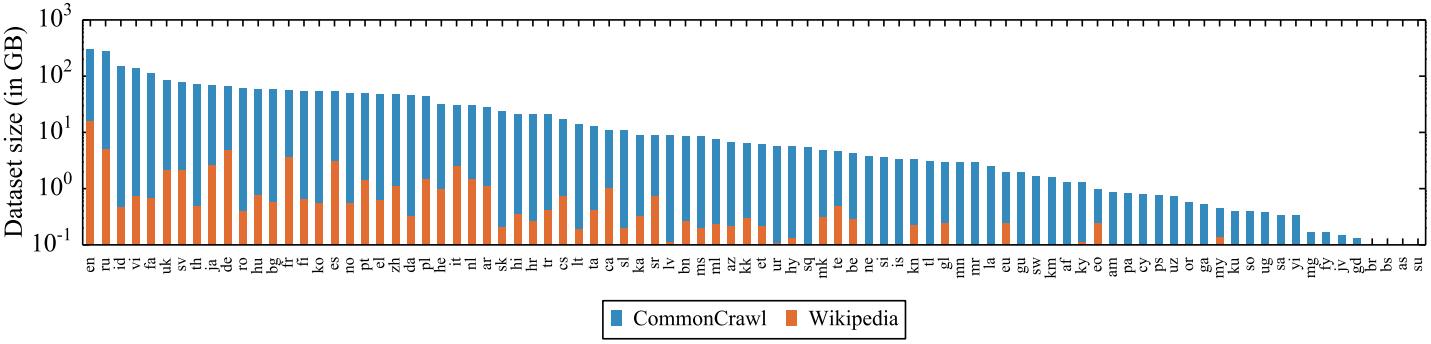
\includegraphics[width=1\textwidth]{resources/data_xlm_r.png}
            \caption{Perbedaan data mBERT (Wikipedia) dengan XLM-R (CC) \parencite{Conneau_XLMR}}
            \label{fig:data_xlm_r}
        \end{figure}

        Penambahan data dan penyeimbangan persentasenya ini terbukti meningkatkan performa model dalam berbagai permasalahan klasifikasi, terutama di bahasa yang sebelumnya memiliki lebih sedikit data. Hal ini dibuktikan dari performa model pada tolak ukur XNLI. Model XLM-R Large berhasil mendapatkan performa terbaik dalam seluruh bahasa tolak ukur XNLI. Bahkan meningkat jauh dari penelitian \parencite{LampleConneau2019} sebelumnya. Peningkatan paling nampak pada bahasa yang memiliki sumber daya sedikit.

\section{Metrik Evaluasi}
Metrik yang digunakan mengacu pada penelitian terkait sebelumnya agar dapat dibandingkan. Untuk mengevaluasi performa klasifikasi ujaran kebencian, digunakan akurasi. Sedangkan untuk mengevaluasi performa dari analisis sentimen yang dilakukan pada bahasa Indonesia, digunakan \textit{f1-score}. \textit{f1-score} adalah rata-rata harmonis antara \textit{precision} dan \textit{recall}. 

Precision merupakan rasio prediksi benar positif dibandingkan dengan keseluruhan hasil yang diprediksi positif. Precision menjawab pertanyaan " Berapa persen teks yang benar memiliki sentimen positif dari keseluruhan mahasiswa yang diprediksi memiliki sentimen positif". Definisi dari \textit{precision} secara matematis dapat dilihat pada persamaan \ref{eq:precision}.
\begin{equation}
    precision=\frac{True Positive}{True Positive + False Positive}
    \label{eq:precision}
\end{equation}

Recall merupakan rasio prediksi benar positif dibandingkan dengan keseluruhan data yang benar positif. Recall menjawab pertanyaan "Berapa persen teks yang diprediksi memiliki sentimen positif dibandingkan keseluruhan teks yang sebenarnya memiliki sentimen positif". Definisi dari \textit{recall} secara matematis dapat dilihat pada persamaan \ref{eq:recall}.
\begin{equation}
    recall=\frac{True Positive}{True Positive + False Negative}
    \label{eq:recall}
\end{equation}

Sehingga terakhir, definisi dari \textit{f1-score} secara matematis dapat dilihat pada persamaan \ref{eq:f1-score}. 
\begin{equation}
    f1-score=2.\: \frac{precision\: .\: recall}{precision+recall}
    \label{eq:f1-score}
\end{equation}

Dengan pengelompokkan prediksi sesuai dengan \textit{confusion matrix} pada tabel \ref{tab:confusion_matrix}.
\begin{table}[ht]
    \centering
    \begin{tabular}{@{}cc|cc@{}}
    \multicolumn{1}{c}{} &\multicolumn{1}{c}{} &\multicolumn{2}{c}{Prediksi} \\ 
    \multicolumn{1}{c}{} & 
    \multicolumn{1}{c|}{} & 
    \multicolumn{1}{c}{\textit{True}} & 
    \multicolumn{1}{c}{\textit{False}} \\ 
    \cline{2-4}
    \multirow[c]{2}{*}{\rotatebox[origin=tr]{90}{Label}}
    & \textit{True}  & \textit{True Positive} & \textit{False Negative}   \\[1.5ex]
    & \textit{False}  & \textit{False Positive}   & \textit{True Negative} \\ 
    \cline{2-4}
    \end{tabular}
    \caption{Tabel \textit{Confusion matrix}.}
    \label{tab:confusion_matrix}
\end{table}

\section{Penelitian Terkait}
Sebelumnya belum terdapat penelitian, dalam bahasa apapun, yang memanfaatkan dan menganalisa pengaruh penggunaan \textit{multilingual language model} untuk menambah data pelatihan dalam permasalahan analisis sentimen dan klasifikasi ujaran kebencian. Tetapi dalam permasalahan analisis sentimen dan klasifikasi ujaran kebencian bahasa Indonesia, telah banyak penelitian terkait. Penelitian tersebut adalah \parencite{FarhanKhodra2017}, \parencite{CrisdayantiPurwarianti2019}, dan \parencite{Ibrohim_Budi_2019}. Untuk pemanfaatan \textit{multilingual language model} dalam klasifikasi teks diluar bahasa Indonesia, sudah terdapat penelitian oleh \parencite{LampleConneau2019} dalam permasalahan klasifikasi apakah sebuah pasangan teks berkaitan, kontradiksi, atau netral. 

\textbf{Pada penelitian \parencite{FarhanKhodra2017}} yang berjudul “\textit{Sentiment-specific word embedding for Indonesian sentiment analysis}”, berbagai bentuk representasi teks dibandingkan dan dievaluasi menggunakan dataset ulasan TripAdvisor. Hasil dari penelitian ini dapat dilihat pada Tabel \ref{tab:FarhanKhodra2017}.
\begin{table}[!h]
    \centering
    \caption{Sebagian hasil eksperimen penelitian \parencite{FarhanKhodra2017}.}
    \begin{tabular}{|l|l|l|}
    \hline
    \multicolumn{1}{|c|}{\multirow{2}{*}{\textbf{Word Embedding}}} & \multicolumn{2}{c|}{\textbf{Hasil Evaluasi}}                                                    \\ \cline{2-3} 
    \multicolumn{1}{|c|}{}                                         & \multicolumn{1}{c|}{\textbf{10-fold cross validation}} & \multicolumn{1}{c|}{\textbf{Data Uji}} \\ \hline
    Bag of words                                                   & 0.8345                                                 & 0.8232                                 \\ \hline
    TF-IDF                                                         & \textbf{0.8492}                                        & \textbf{0.8521}                        \\ \hline
    % Word2Vec                                                       & 0.7204                                                 & 0.7219                                 \\ \hline
    % SSWE dari W2V                                                  & 0.7311                                                 & 0.7224                                 \\ \hline
    SSWE                                                           & 0.7623                                                 & 0.7687                                 \\ \hline
    \end{tabular}
    \label{tab:FarhanKhodra2017}
\end{table} 

\textbf{Pada penelitian \parencite{CrisdayantiPurwarianti2019}} yang berjudul “\textit{Improving Bi-LSTM Performance for Indonesian Sentiment Analysis Using Paragraph Vector}”, dilakukan perbandingan berbagai representasi dokumen dan topologi \textit{neural network}. Hasil terbaik didapatkan oleh model yang dilatih pada representasi kata dengan TF-IDF dan representasi paragraf dengan Doc2vec. Model Bi-LSTM yang dilatih berhasil mendapatkan F1-Score sebesar 0.9369 pada data sentimen dari berbagai media sosial (Twitter, Zomato, TripAdvisor, Facebook, Instagram, Qraved). Hasil dari penelitian ini dapat dilihat pada Tabel \ref{tab:CrisdayantiPurwarianti2019}.

\begin{table}[!h]
    \centering
    \caption{Hasil penelitian \parencite{CrisdayantiPurwarianti2019}.}
    \begin{tabular}{|l|l|l|l|}
    \hline
    \multicolumn{1}{|c|}{\textbf{Model}} & \multicolumn{1}{c|}{\textbf{Precision}} & \multicolumn{1}{c|}{\textbf{Recall}} & \textbf{F1-Score} \\ \hline
    SVM (TF-IDF)                         & 0.7977                                  & 0.8878                               & 0.8658            \\ \hline
    Bi-LSTM (WE)                         & 0.9166                                  & 0.9126                               & 0.9125            \\ \hline
    Bi-LSTM (PV+WE)                      & \textbf{0.9384}                         & \textbf{0.9369}                      & \textbf{0.9369}   \\ \hline
    \end{tabular}
    \label{tab:CrisdayantiPurwarianti2019}
\end{table}

\textbf{Pada penelitian \parencite{Ibrohim_Budi_2019}} yang berjudul "\textit{Multi-label Hate Speech and Abusive Language Detection in Indonesian Twitter}", dilakukan klasifikasi multi-label ujaran kebencian \& kasar. Dataset ujaran kebencian \& kasar tersebut merupakan \textit{tweet} dari sosial media Twitter\footnote{\url{https://www.twitter.com/}} yang dianotasi oleh 30 anotator dengan berbagai etnis, agama, dan pekerjaan. 

Terdapat dua skenario eksperimen yang dicoba. Pada skenario pertama, klasifikasi dilakukan hingga ke target, kategori, dan levelnya. Pada skenario kedua, klasifikasi hanya dilakukan sampai menentukan kategori teks ujaran kebencian atau kasar saja. Skenario kedua ini lah yang paling dekat dengan tugas akhir ini. Dalam eksperimennya, metrik yang diperhatikan adalah rata-rata dari akurasi prediksi terhadap masing-masing label. Hasil skenario kedua dapat dilihat pada Tabel \ref{tab:Ibrohim_Budi_2019_2}

\begin{table}[hbt]
    \centering
    \caption{Hasil klasifikasi ujaran kebencian \parencite{Ibrohim_Budi_2019}.}
    \begin{tabular}{|l|l|l|}
    \hline
    \textbf{Tipe Fitur} & \textbf{Fitur Terbaik} & \textbf{Rata-rata Akurasi (\%)} \\ \hline
    word n-gram              & word unigram                                    & 73.53                          \\ \hline
    character n-gram         & character quadgrams                             & 72.44                          \\ \hline
    ortography               & exclamation mark                                & 45.27                          \\ \hline
    lexicon                  & positive sentiment + abusive lexicon            & 52.10                          \\ \hline
    \end{tabular}
    \label{tab:Ibrohim_Budi_2019_2}
\end{table}

\begin{table}[!h]
    \centering
    \caption{Hasil pada uji akurasi di dataset XNLI \parencite{LampleConneau2019}.}
    \begin{tabular}{|l|l|l|l|l|}
    \hline
    \multicolumn{1}{|c|}{\textbf{Evaluasi \textit{Sentence Encoder} Lintas Bahasa}} & \multicolumn{1}{c|}{\textbf{en}} & \multicolumn{1}{c|}{\textbf{fr}} & \textbf{es}   & \textbf{de}   \\ \hline
    \parencite{LamplePhrase2018}                            & 73.7                             & 67.7                             & 68.7          & 67.7          \\ \hline
    \parencite{Devlin_Chang_Lee_Toutanova_2019}         & 81.4                             & -                                & 74.3          & 70.5          \\ \hline
    \parencite{Artetxe_Schwenk_2019}                      & 73.9                             & 71.9                             & 72.9          & 72.6          \\ \hline
    \parencite{LampleConneau2019}                           & \textbf{83.2}                    & \textbf{76.5}                    & \textbf{76.3} & \textbf{74.2} \\ \hline
    \end{tabular}
    \label{tab:LampleConneau2019}
\end{table}

\textbf{Pada penelitian \parencite{LampleConneau2019}} yang berjudul “\textit{Cross-lingual Language Model Pretraining}”, model berarsitektur \textit{transformer} dilatih dengan MLM dan \textit{shared sub-word vocabulary} pada data Wikipedia. Kemudian keluaran dari \textit{layer} terakhir model ini menjadi masukan ke \textit{layer} linier terakhir. Model mereka berhasil memecahkan beberapa state-of-the-art pada  dataset tolak ukur klasifikasi pembelajaran lintas bahasa XNLI \parencite{Conneau_Rinott_Lample_Williams_Bowman_Schwenk_Stoyanov_2018}. Hasil dari penelitian ini dapat dilihat pada Tabel \ref{tab:LampleConneau2019}. Hasil yang ditampilkan hanya 4 dari 15 bahasa dan hanya hasil XLM dengan pendekatan \textit{unsupervised}.



